\chapter{Artificial Neural Networks}



Artificial neural networks are the extension from traditional machine learning models into deep learning methods.

(rewrite this into and place figures somewhere later, or in the section of working with structured/unstructured data)

A common elementary application is to utilize a network to recognize and classify image date based on the pixel values, as is shown in Figure \ref{minecraft}.  In image data, each pixel is an input value determined by a number corresponding to that specific color.  For grayscale image data, that number is a value from 0 to 1.  Color images are represented as vectors of three values (RGB).

\begin{figure}[H]
    \centering
    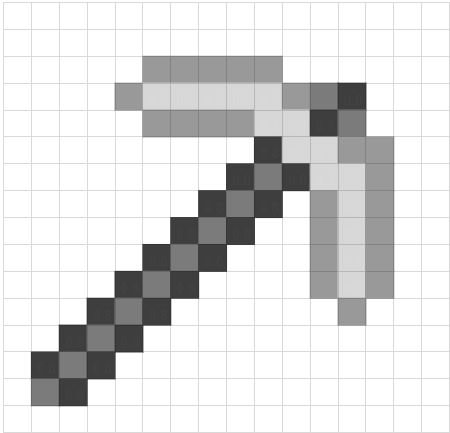
\includegraphics[width=.35\textwidth]{Figures/pickaxe_1.png}
    \hspace{30pt}
    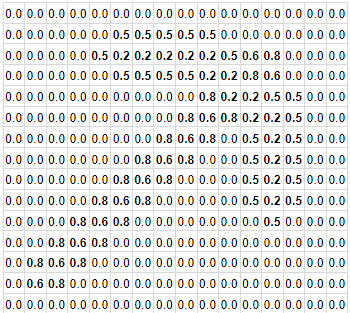
\includegraphics[width=.35\textwidth]{Figures/pickaxe_2.png}
    \caption{\footnotesize{An 16x16 pixel image, with its numerical counterpart next to it.  In greyscale image data, a value of 0.0 corresponds to white, 1.0 to black, and ordered variations of gray to values in between}}
    \label{minecraft}
\end{figure}

Classification tasks vs. regression tasks

Of course, image data is not the only data that a neural network can be used on.  Any type of data can be modeled with a neural network, provided there is enough of it to match the complexity if the model.  Image data tends to have a great number of inputs to begin with.  What makes these deep learning models particularly useful is that they identify non-linear patterns, and with more abstraction than traditional machine learning algorithms like K-Nearest Neighbors or Naive Bayes.



\section{The Architecture of Neural Networks} %-------------SECTION

Hint toward issues like overfitting, but elaborate more in section 2.3.

- Also, first mention \textbf{Optimization} here

%---Pathway to Architecture file---
\subfile{Architecture}  

%\subsection{Gradient Descent}

%\subsubsection{Simulation in R}

%\subsection{Backpropagation}

%\subsubsection{Simulation in R}

\subsection{More Optimization Algorithms}

Aside from Gradient Descent.

Describe Stochastic Gradient Descent in subtle detail.

Make mention of other optimization algorithms (Adam, Adagrad, RMSprop), with only a brief description of them.  Only make mention of the ones to be used in Keras during practical examples in the next section.

\section{Types of Neural Networks} %-------------SECTION
The previous section described a \textbf{Multi-Layer Perceptron} network.  This section is devoted to other network types and their most practical uses.

%Write this up in R following along the code from %\textbf{RAI}, with supplementary information from %other sources as well.  

Obviously not all types will be covered, but here are a few.  

Include \textbf{mathematical notation} for each network mentioned.

%\subsection{Multi-Layer Perceptron}
%Keras Model: "sequential"
%This ws described above

\subsection{Convolutional Neural Networks}
Unstructured image data

\subsection{Generative Adversarial Networks}
Unstructured image data

Image generation to try and fool a "discriminator" network

\subsection{Recurrent Neural Networks}
Unstructured text data

NLP/translation/text generation
Time series forecasting

\subsection{Long Short-Term Memory Network}
Unstructured text data

\subsection{Convolutional Recurrent Networks}
Unstructured text data

\section{Techniques to Improve Model Performance} %-------------SECTION

The primary objective in machine learning (and therefore deep learning) is to perform well on new, unseen data. 

- \textbf{Overfitting} and \textbf{underfitting}

\subsection{Rating Model Performance}
- \textbf{Generalization}
- \textbf{Training error}  
- \textbf{Generalization error} (test error)

\subsection{Addressing Model Performance}
- \textbf{Capacity}
- \textbf{Regularization}

\subsection{Common Problems and Relevant Techniques}

Earthquake example